\documentclass[final]{beamer}
\usefonttheme{serif}
\mode<presentation>{\usetheme{ASU}}
\usepackage{amsmath, amsfonts, amssymb, pxfonts, eulervm, xspace, enumerate, hyperref, color, bookmark}
\usepackage{graphicx}
\usepackage[orientation=landscape, size=a0, scale=1.4, debug]{beamerposter}
%\usepackage{natbib}

\usecolortheme{rose}
%\setbeamercolor{background canvas}{bg=magenta!16!yellow!90}

%\beamertemplategridbackground[1cm]

%-- Header and footer information ----------------------------------
\newcommand{\footright}{\href{https://github.com/STAT-ATA-ASU/STT3851Spring2016}{https://github.com/STAT-ATA-ASU/STT3851Spring2016}}
\newcommand{\footleft}{\href{mailto:arnholtat@appstate.edu}{Faculty Advisor: Alan Arnholt}}

\def\conference{STT 3851: Statistical Data Analysis II}
\title{Predicting Housing Prices in King County, WA}
\author{Andrew Sullivan, Tucker Southern, Hannah Laws} 
\institute{Department of Mathematical Sciences}
%-------------------------------------------------------------------


%-- Main Document --------------------------------------------------
\usepackage{Sweave}
\begin{document}
\Sconcordance{concordance:Poster.tex:Poster.Rnw:%
1 25 1 1 0 5 1 1 22 97 1 1 5 %
17 1}

\begin{frame}[fragile]
\vspace{-2ex}
\begin{columns}[t]


%-- Column 1 ---------------------------------------------------
\begin{column}{0.31\linewidth}
\begin{minipage}[t][.955\textheight]{\linewidth} 
%-- Block 1-1
\vspace{0ex}
\begin{block}{Overview}
\begin{itemize}
\item The goal of this project was to predict prices for houses in King County, Washington.
\item Data was examined from 17384 houses sold in the county between 2014 and 2015 in order to construct a pricing model.
\item Models were constructed through exploratory analysis and forward AIC selection, and then tested using K-fold cross-validation.
\item All computations and graphs are created with the open source software \texttt{R} \cite{R-base}. 
\end{itemize}

\centering
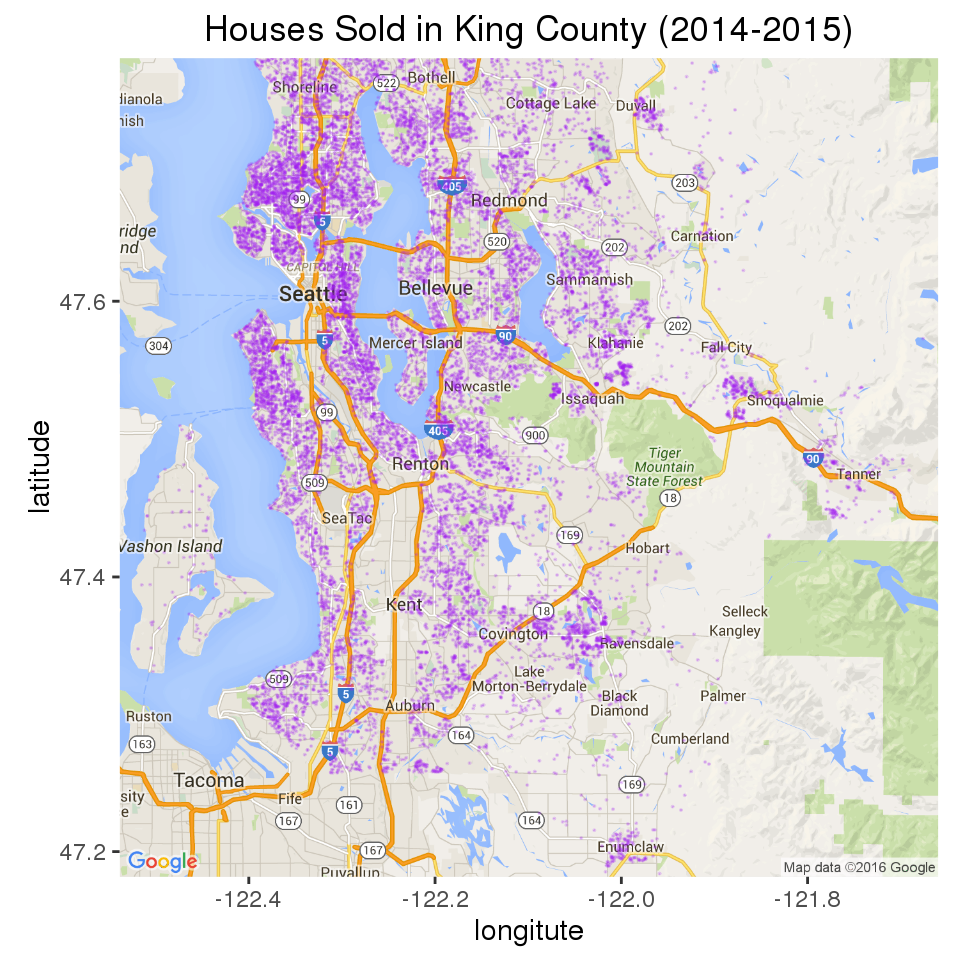
\includegraphics{countymap.png}
\vspace{0ex}
\end{block}
\vfill

%-- Block 1-2
\vspace{0ex}
\begin{block}{Data Formatting}
\begin{itemize}
\item The variables $Waterfront$, $Condition$, $Grade$, and $Zipcode$ were converted from numeric values to factors.
\item The variable $YearRenovated$ was set to the corresponding $YearBuilt$ for any houses that were missing $YearRenovated$ values - that is, any houses that had not been renovated had their renovation dates re-set to the dates they were originally built.
\item The variables $Grade$ and $Condition$ were collapsed to account for limited observations and limited distinct effect in their lower categories.
\item Finally, a new variable, $LotSize$, was introduced based on established realtor lot categories \cite{pardoe_modeling_2008}.
\end{itemize}
\vspace{0ex}
\end{block}
\vfill

\end{minipage}
\end{column}%1

%-- Column 2 ---------------------------------------------------

\begin{column}{0.31\linewidth}
\begin{minipage}[t][.955\textheight]{\linewidth} 
%-- Block 2-1
\begin{block}{Exploratory Analysis}
\begin{itemize}
\item Exploratory analysis was performed by examining plots and single-variable regressions for various variables on to $Price$, as well as variable interactions which were assumed to be significant (such as the interaction between $Bedrooms$ and $Bathrooms$ on to $Price$) \cite{james_introduction_2013}. 
\item Variables and interactions which looked to have strong correlation were later added to the model and tested for significance.
\item The boxplot below shows the effect of waterfront location on house price:
\end{itemize}

\centering
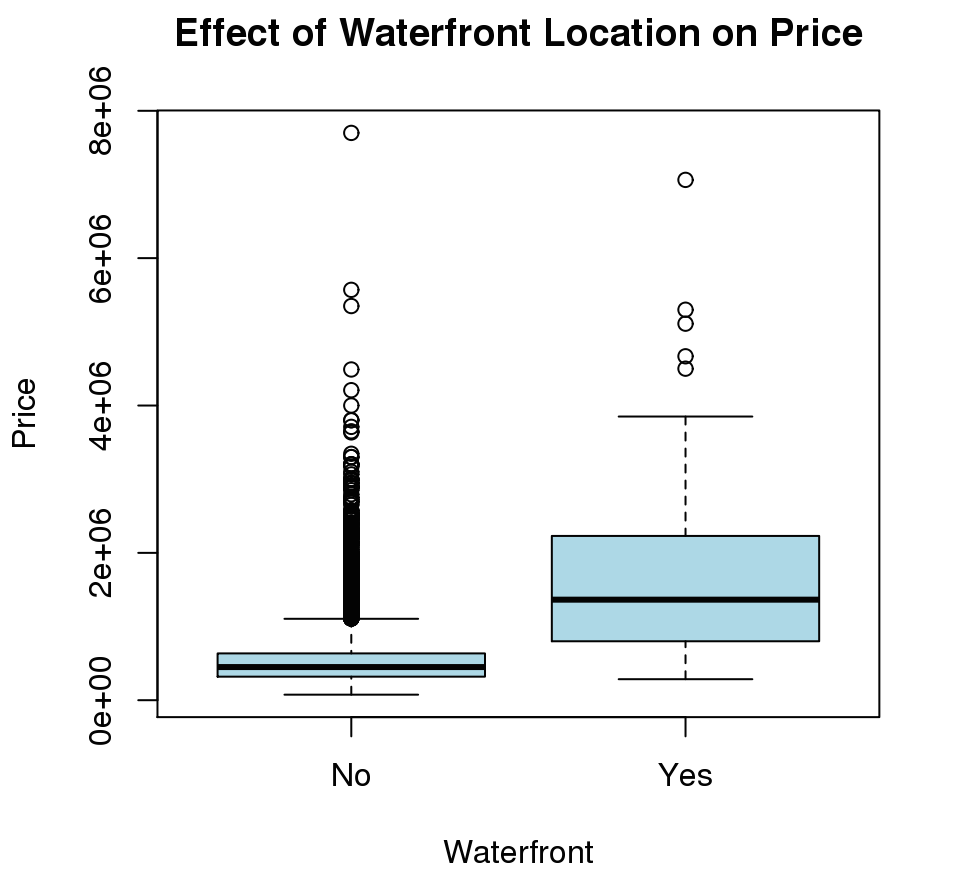
\includegraphics{waterfront.png}
\vspace{0ex}
%\centering
%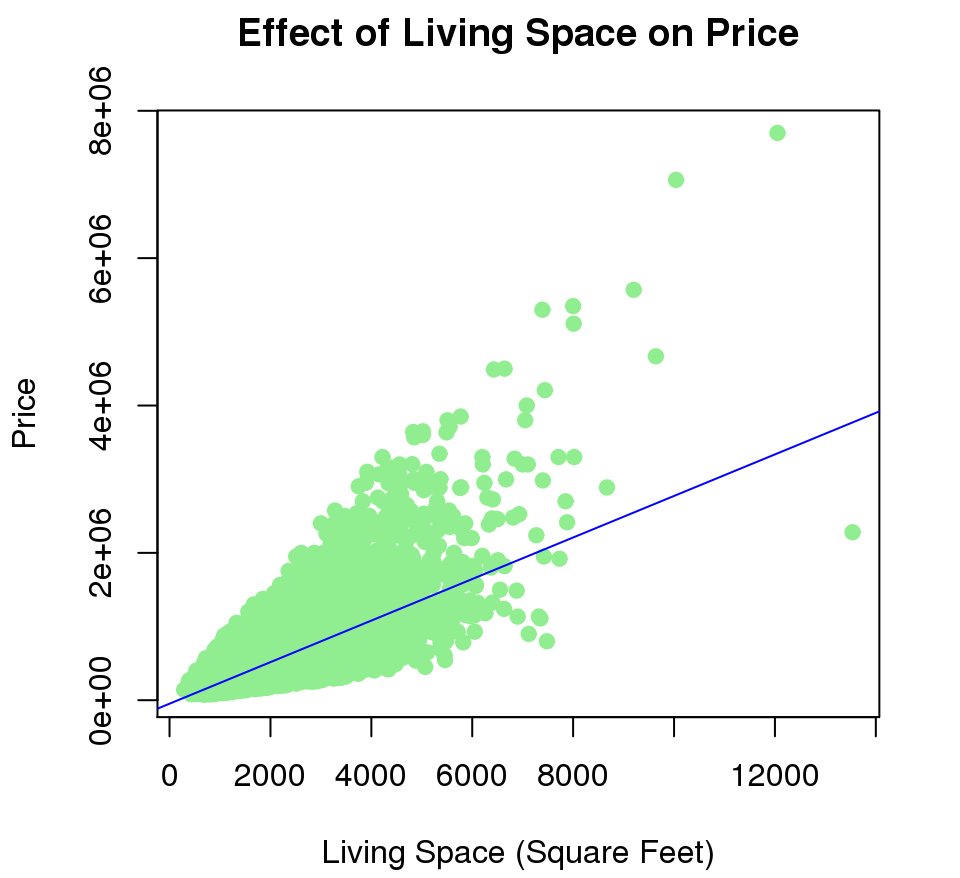
\includegraphics{sqftliving.png}
%\vspace{0ex}
\end{block}
\vfill

%-- Block 2-2
\begin{block}{Model Creation}
\begin{itemize}
\item The first model was created by comparing AIC in a forward stepwise algorithm \cite{R-MASS}.
\item The second model included polynomials based on residual plots of the forward-selected model \cite{R-car}, and interaction terms based on exploratory analysis.
\item The final model was a simplified version of the second, dropping features with low significance. It included these features and interactions: $E(price) = b_0 + b_1 Grade + b_2 Zipcode + b_3 SqftLiving^2 + b_4 Waterfront$
$+ b_5 View + b_6 LotSize + b_7 Condition + b_7 SqftAbove^2 + b_8 YearBuilt$
$+ b_9 YearRenovated + b_10 Floors + b_11 SqftLiving15 + b_12 SqftLot15$
$+ b_13 (SqftLiving:SqftLot) + b_15 (Bedrooms:Bathrooms)$
$+ b_16 (Waterfront:SqftLiving) + b_17 (Waterfront:SqftLot)$
$+ b_18 (Lat:Long) + b_19 (Zipcode:SqftLiving)$
\end{itemize}
\vspace{0ex}
\end{block}
\vfill

\end{minipage}
\end{column}%2

%-- Column 3 ---------------------------------------------------
\begin{column}{0.31\linewidth}
\begin{minipage}[t][.955\textheight]{\linewidth} 
%-- Block 3-1
\begin{block}{Model Selection}
\begin{itemize}
\item We used 5-fold cross-validation to select the best model \cite{R-boot}. The simplified final model consistently performed the best, having the lowest mean squared test error.
\item Results of ten repetitions of cross-validation on all three models are plotted below:
\end{itemize}

\centering
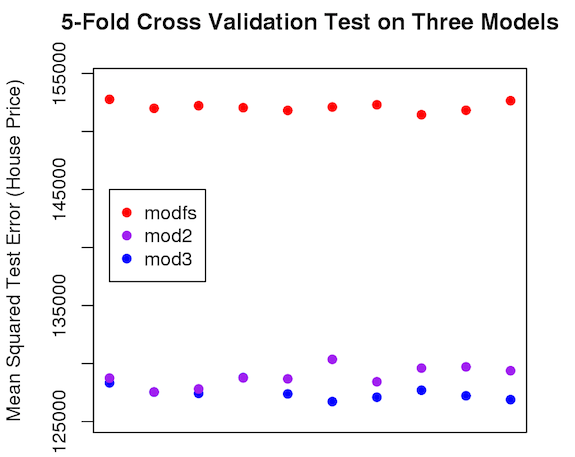
\includegraphics{cvplot.png}
\vspace{0ex}
\end{block}
\vfill


%-- Block 3-2
\begin{block}{References}
\footnotesize
\setbeamertemplate{bibliography item}[text]
\vspace{-1ex}

\bibliographystyle{plain}  % can use plain but comment out natbib at top if using plain
\bibliography{PackagesUsed.bib,CV.bib}
%\normalsize
\vfill
\end{block} 
\vfill

\end{minipage}
\end{column}%3




\end{columns}
\end{frame}
\end{document}

